% ============================================================
%  第三卷 第五章 有心力场中的运动（§32–§37 + 习题）
%  底本：高教社中文版第6版（严肃译）；OCR 错误已修正，脚注文本待从纸版补录
%
%  已修正的 OCR / 原书错误（对照原书页面 PNG 逐条核实）：
%  1. §32 (32.13)：OCR 丢失第二行字母，按原书 p109 补齐 s p d f g h i k；
%  2. §32：OCR 将脚注①内两式（p̂_r、Ĥ 的表式）误并入正文，已从正文删除，
%     并按原书 p108 归位为该处脚注（脚注代理核录）；
%  3. §33 正文"作替换 χ′_kl=η_{k,l+1}"按原书 p111 为 χ′_kl=rχ_{k,l+1}；
%     "球人射波"→"球入射波"；
%  4. §33 习题4 式(2)：原书 p116 将 F 首参量印作 −n/2−l/2，按径量子数
%     n_r=(n−l)/2 及 1p、1d 态（n_r=0）径向无节点的要求，修正为 −n/2+l/2；
%  5. §34 ψ 展开式：原书 p118 系数印作 1/(ik)，经与(34.1)+(33.9)推导核对
%     （出射波渐近匹配、原点附近逐项匹配两法一致），应为 i^l/(ik)=i^{l−1}/k，
%     原书漏排 i^l，σ_l=(π/k²)(2l+1) 不受影响；
%  6. §36 (36.24) 前一式：OCR 之 Π_{s=1}^n → Π_{s=1}^l、e^{−2πk} → e^{−2π/k}；
%  7. §36 (36.29)：OCR 乱码"=λv/13−…"按原书 p127 为"=常数"；
%  8. §37 (37.15)：OCR 之减号系排版噪声，按原书 p120 为三因子乘积；
%  9. 习题内编号公式按原书每题自成 (1),(2),…，用 \setcounter{equation}{0}
%     与局部 \theequation 实现节末恢复（main.tex 不变）；
%  10. 其它：U_0（OCR 作 U_。/U_𝔬）、(36.13) e^{−ν/n}→e^{−r/n}、§36 习题4
%      ξR′→ξR″、E_ν→E_n、r^{2(1+1)}→r^{2(l+1)}、ψ~r^ι→ψ~r^l、
%      按−1/r^3→按−1/r^s、cos′θ→cos^l θ、(2l)!/2^l(l!)²、
%      函数名正体收紧（\sin,\cos,\cot,\sinh,\ln,\arg,\exp）、\mathrm{d} 收紧等。
%  11. 脚注转录备忘（脚注代理）：p125 脚注①原书印作 ρ=−2ik/r，应为 ρ=−2ikr
%      （ρ=2ikr 的复共轭，量纲核对亦否证 /r），已改正；p112 脚注②"同宇称"
%      系原书原文照录；其余脚注均按 pages300/pages 原书页面忠实转录。
%
%  遗留问题（OCR 存疑，已照原书排版）：
%  - (33.8) 递推式 χ_{k,l+1}=χ′_kl/r 与 (33.9) 之间逐级差因子 (−1/k)^l，
%    原书如此——(33.9) 前因子 k^{−l} 书中明言"为归一化目的而引进"（p98）；
%  - §33 习题1 解中"令 α=ħ/√(2ma²U₀)"OCR 作 h/√…，按原书 p101 为 ħ；
%  - (33.5) 引用"(5.14)"、(33.6) 解引用"(21.9)"照 OCR 与原书页面保留。
% ============================================================
\chapter{有心力场中的运动}

\section{有心力场中的运动}

量子力学中两个相互作用粒子的运动问题，可以照经典力学中所做的那样，把它简化成为一个单粒子问题.按 $U(r)$ 规律（$r$ 为这两个粒子间的距离）相互作用着的两个粒子（质量分别为 $m_1,m_2$），其哈密顿量呈以下形式：
\begin{equation}
  \hat{H}=-\frac{\hbar^2}{2m_1}\Delta_1-\frac{\hbar^2}{2m_2}\Delta_2+U(r),
\end{equation}
式中 $\Delta_1$ 和 $\Delta_2$ 分别是这两个粒子坐标的拉普拉斯算符.我们引进新变量 $\boldsymbol{R}$ 和 $\boldsymbol{r}$，代替粒子的径矢 $\boldsymbol{r}_1$ 和 $\boldsymbol{r}_2$：
\begin{equation}
  \boldsymbol{r}=\boldsymbol{r}_2-\boldsymbol{r}_1,\qquad
  \boldsymbol{R}=\frac{m_1\boldsymbol{r}_1+m_2\boldsymbol{r}_2}{m_1+m_2};
\end{equation}
$\boldsymbol{r}$ 为两粒子距离矢量，而 $\boldsymbol{R}$ 为质心的径矢.经过简单计算后，可得
\begin{equation}
  \hat{H}=-\frac{\hbar^2}{2(m_1+m_2)}\Delta_R-\frac{\hbar^2}{2m}\Delta+U(r)
\end{equation}
式中 $\Delta_R$ 和 $\Delta$ 分别是对 $\boldsymbol{R}$ 和 $\boldsymbol{r}$ 坐标的拉普拉斯算符，$m_1+m_2$ 是该系统的总质量，而 $m=m_1m_2/(m_1+m_2)$ 是约化质量.由此可见哈密顿量变成了两个独立部分之和.与此相应，我们可以把 $\psi(\boldsymbol{r}_1,\boldsymbol{r}_2)$ 写成 $\varphi(\boldsymbol{R})\psi(\boldsymbol{r})$ 的乘积形式，其中的 $\varphi(\boldsymbol{R})$ 函数描述质心的运动（如同质量为 $m_1+m_2$ 的一个自由粒子），而 $\psi(\boldsymbol{r})$ 函数描述这两个粒子的相对运动［如同质量为 $m$ 的一个粒子在有心力场 $U(r)$ 中运动］.

一个粒子在有心力场中运动时薛定谔方程具有下列形式：
\begin{equation}
  \Delta\psi+\frac{2m}{\hbar^2}\left[E-U(r)\right]\psi=0.
\end{equation}
采用拉普拉斯算符在球坐标中的熟知表式，我们可以把上式写成
\begin{equation}
\begin{aligned}
  &\frac{1}{r^2}\frac{\partial}{\partial r}\left(r^2\frac{\partial\psi}{\partial r}\right)
  +\frac{1}{r^2}\left[\frac{1}{\sin\theta}\frac{\partial}{\partial\theta}
  \left(\sin\theta\frac{\partial\psi}{\partial\theta}\right)
  +\frac{1}{\sin^2\theta}\frac{\partial^2\psi}{\partial\varphi^2}\right]+\\
  &\quad+\frac{2m}{\hbar^2}\left[E-U(r)\right]\psi=0.
\end{aligned}
\end{equation}
如果在式中引入(26.16)式的角动量平方算符 $\hat{l}^2$，可得\footnote{如果引入动量的径向分量算符 $\hat{p}_r$，它的形状为 $\hat{p}_r\psi=-i\hbar\frac{1}{r}\frac{\partial}{\partial r}(r\psi)=-i\hbar\left(\frac{\partial}{\partial r}+\frac{1}{r}\right)\psi$，则哈密顿量就可以写成下列形式：$\hat{H}=\frac{1}{2m}\left(\hat{p}_r^2+\hbar^2\hat{l}^2/r^2\right)+U(r)$，这和经典哈密顿函数的球坐标形式完全相同.}
\begin{equation}
  \frac{\hbar^2}{2m}\left[-\frac{1}{r^2}\frac{\partial}{\partial r}
  \left(r^2\frac{\partial\psi}{\partial r}\right)+\frac{\hat{l}^2}{r^2}\psi\right]+U(r)\psi=E\psi.
\end{equation}
在有心力场中运动时，角动量是守恒的.我们来考虑角动量 $l$ 及其分量 $m$ 都有定值的那些定态.这两个值确定了波函数的角部.因此我们要找的(32.6)式之解具有下列形式：
\begin{equation}
  \psi=R(r)\mathrm{Y}_{lm}(\theta,\varphi),
\end{equation}
式中的 $\mathrm{Y}_{lm}(\theta,\varphi)$ 是球谐函数.

由于 $\hat{l}^2\mathrm{Y}_{lm}=l(l+1)\mathrm{Y}_{lm}$，我们得到径向函数 $R(r)$ 的方程式：
\begin{equation}
  \frac{1}{r^2}\frac{\mathrm{d}}{\mathrm{d}r}\left(r^2\frac{\mathrm{d}R}{\mathrm{d}r}\right)
  -\frac{l(l+1)}{r^2}R+\frac{2m}{\hbar^2}\left[E-U(r)\right]R=0.
\end{equation}
上式根本不包含数值 $l_z=m$，这与能级对角动量方向的简并度为 $(2l+1)$ 是一致的，这一点我们已经熟悉.

我们来研究波函数的径部.作下列变换
\begin{equation}
  R(r)=\frac{\chi(r)}{r},
\end{equation}
(32.8)式变成下列形式：
\begin{equation}
  \frac{\mathrm{d}^2\chi}{\mathrm{d}r^2}
  +\left[\frac{2m}{\hbar^2}(E-U)-\frac{l(l+1)}{r^2}\right]\chi=0
\end{equation}
如果势场 $U(r)$ 处处有限，波函数 $\psi$ 在整个空间也必须处处有限，包括原点在内，从而其径部 $R(r)$ 也必处处有限.根据这一点 $\chi(r)$ 在 $r=0$ 处必须等于零：
\begin{equation}
  \chi(0)=0.
\end{equation}
如果 $r\to0$ 时势场趋向无穷大，上述条件实际上还是成立的（见§35）.

(32.10)式在形式上等同于具有下列势场的一维运动薛定谔方程：
\begin{equation}
  U_l(r)=U(r)+\frac{\hbar^2}{2m}\frac{l(l+1)}{r^2},
\end{equation}
它是势能 $U(r)$ 与下式之和：
\begin{equation*}
  \frac{\hbar^2l(l+1)}{2mr^2}=\frac{\hbar^2\hat{l}^2}{2mr^2},
\end{equation*}
这个表式可以称为离心能.由此可见，有心力场中的运动问题，可以归结为运动区域在一端受限制的（$r=0$ 处的边界条件）一个一维运动问题.$\chi$ 函数的归一化条件也是“一维”的，由下列积分确定：
\begin{equation*}
  \int_0^{\infty}|R|^2r^2\,\mathrm{d}r=\int_0^{\infty}|\chi|^2\,\mathrm{d}r.
\end{equation*}

一端受限的一维运动，其能级是非简并的（§21）.因此我们可以这样说，如果能量已经给定，则(32.10)式之解，亦即波函数的径部，就被完全确定.如果还记得这个波函数的角部已由 $l$ 和 $m$ 值完全确定，我们就得到这样的结论，对有心力场中的运动讲来，它的波函数可以由 $E$，$l$ 和 $m$ 三个数值完全确定.换句话说，对这样的运动讲来，能量，角动量的平方以及角动量的 $z$ 分量这三个量组成物理量的一个完全集.

有心力场中的运动问题归结为一维问题后，使我们有可能应用振荡定理（见§21）.我们把具有给定 $l$ 值的各个能量本征值（离散谱）按递增次序加以排列，给予编号 $n_r$，令最低能级的编号为 $n_r=0$.则 $n_r$ 确定了波函数的径部在 $r$ 的有限值域内所具有的节点数（$r=0$ 点除外）.$n_r$ 称为径量子数.对有心力场中的运动讲来，$l$ 常常称为角量子数，$m$ 则称为磁量子数.

对于角动量 $l$ 值不同的各种粒子态，有一套常用符号；用下列拉丁字母标志：
\begin{equation}
\begin{array}{c*{9}{@{\quad}c}}
  l={}&0&1&2&3&4&5&6&7&\cdots\\
   &\mathrm{s}&\mathrm{p}&\mathrm{d}&\mathrm{f}&\mathrm{g}&\mathrm{h}&\mathrm{i}&\mathrm{k}&\cdots
\end{array}
\end{equation}
运动于有心力场中的一个粒子，它的基态总是 s 态；因为如果 $l\neq0$，则波函数的角部一定具有节点，但是基态波函数根本不存在节点.我们还可以断言，$l$ 给定后，能量的最小可能值随 $l$ 增加.因为角动量的存在使哈密顿量中多出一个正项 $\hbar^2l(l+1)/2mr^2$，这一项是随 $l$ 增加的.

现在来找径函数在原点附近的形状.此处我们假定
\begin{equation}
  \lim_{r\to0}U(r)r^2=0.
\end{equation}
我们把 $R(r)$ 表成 $r$ 的幂级数，当 $r$ 很小时只保留该级数的首项；换句话说，我们把 $R(r)$ 表成 $R=\text{常数}\times r^s$ 的形式.把它代入下列方程中：
\begin{equation*}
  \frac{\mathrm{d}}{\mathrm{d}r}\left(r^2\frac{\mathrm{d}R}{\mathrm{d}r}\right)-l(l+1)R=0,
\end{equation*}
这个式子是由(32.8)式乘以 $r^2$ 后再取极限 $r\to0$ 得到的，结果得
\begin{equation*}
  s(s+1)=l(l+1).
\end{equation*}
故
\begin{equation*}
  s=l\quad\text{或}\quad s=-(l+1).
\end{equation*}
$s=-(l+1)$ 这个解不满足必要条件；$r=0$ 时它变成无穷大（注意 $l\geqslant0$）.因此只留下 $s=l$ 这个解，也就是说，具有给定 $l$ 值的状态波函数在原点附近和 $r^l$ 成正比：
\begin{equation}
  R_l\approx\text{常数}\times r^l.
\end{equation}
粒子与原点的距离在 $r$ 和 $r+\mathrm{d}r$ 范围内的概率由 $r^2|R|^2$ 确定，因而和 $r^{2(l+1)}$ 成正比.可见 $l$ 值愈大，这个概率在原点愈快地趋于零.

\section{球面波}

平面波
\begin{equation*}
  \psi_{\boldsymbol{p}}=\text{常数}\times\mathrm{e}^{(i/\hbar)\boldsymbol{p}\cdot\boldsymbol{r}}
\end{equation*}
描述一个定态，该态中一个自由粒子具有确定的动量 $\boldsymbol{p}$（以及确定的能量 $E=p^2/2m$）.现在考虑自由粒子的另一种定态，该态中，不但具有确定的能量值，而且具有确定的角动量绝对值及其分量值.为方便计，我们引入波数 $k$ 代替能量：
\begin{equation}
  k=\frac{p}{\hbar}=\frac{\sqrt{2mE}}{\hbar}.
\end{equation}
角动量为 $l$ 而其投影值为 $m$ 的状态波函数具有下列形式：
\begin{equation}
  \psi_{klm}=R_{kl}(r)\mathrm{Y}_{lm}(\theta,\varphi),
\end{equation}
其中的径函数由下式确定：
\begin{equation}
  R''_{kl}+\frac{2}{r}R'_{kl}+\left[k^2-\frac{l(l+1)}{r^2}\right]R_{kl}=0
\end{equation}
［即(32.8)式中 $U(r)\equiv0$］.连续谱（对 $k$ 而言）的 $\psi_{klm}$ 波函数满足下列正交归一化条件：
\begin{equation*}
  \int\psi^*_{k'l'm'}\psi_{klm}\,\mathrm{d}V
  =\delta_{ll'}\delta_{mm'}\delta\left(\frac{k'-k}{2\pi}\right).
\end{equation*}
对不同的 $l,l'$ 和不同的 $m,m'$ 而言的正交性有角部函数加以保证.径函数则必须按下列条件归一化
\begin{equation}
  \int_0^{\infty}r^2R_{k'l}R_{kl}\,\mathrm{d}r
  =\delta\left(\frac{k'-k}{2\pi}\right)=2\pi\delta(k'-k),
\end{equation}
如果我们不是按“$k/2\pi$ 标度”归一化，而是按“能量标度”亦即按下列条件归一化：
\begin{equation*}
  \int_0^{\infty}r^2R_{E'l}R_{El}\,\mathrm{d}r=\delta(E'-E),
\end{equation*}
那么，按照一般公式(5.14)，我们有
\begin{equation}
  R_{El}=R_{kl}\sqrt{\frac{1}{2\pi}\frac{\mathrm{d}k}{\mathrm{d}E}}
  =\frac{1}{\hbar}\sqrt{\frac{m}{2\pi k}}\,R_{kl}
\end{equation}
$l=0$ 时，(33.3)式可写成
\begin{equation*}
  \frac{\mathrm{d}^2(rR_{k0})}{\mathrm{d}r^2}+k^2rR_{k0}=0;
\end{equation*}
上式之解，当 $r=0$ 时取有限值并满足归一化条件(33.4)者［参考(21.9)式］，呈以下形式：
\begin{equation}
  R_{k0}=2\frac{\sin kr}{r}.
\end{equation}
求解 $l\neq0$ 的(33.3)式时，我们作下列替换：
\begin{equation}
  R_{kl}=r^l\chi_{kl}.
\end{equation}
对 $\chi_{kl}$ 我们有方程式
\begin{equation*}
  \chi''_{kl}+\frac{2(l+1)}{r}\chi'_{kl}+k^2\chi_{kl}=0.
\end{equation*}
将上式对 $r$ 求微商，我们得
\begin{equation*}
  \chi'''_{kl}+\frac{2(l+1)}{r}\chi''_{kl}
  +\left[k^2-\frac{2(l+1)}{r^2}\right]\chi'_{kl}=0.
\end{equation*}
作替换 $\chi'_{kl}=r\chi_{k,l+1}$，上式变成
\begin{equation*}
  \chi''_{k,l+1}+\frac{2(l+2)}{r}\chi'_{k,l+1}+k^2\chi_{k,l+1}=0,
\end{equation*}
这实际上正好是 $\chi_{k,l+1}$ 本来应该满足的方程式.可见相邻的 $\chi_{kl}$ 函数满足下列关系：
\begin{equation}
  \chi_{k,l+1}=\frac{1}{r}\chi'_{kl},
\end{equation}
从而有
\begin{equation*}
  \chi_{kl}=\left(\frac{1}{r}\frac{\mathrm{d}}{\mathrm{d}r}\right)^l\chi_{k0},
\end{equation*}
其中的 $\chi_{k0}=R_{k0}$ 已由(33.6)式所确定（该式当然可以乘一任意常数）.

就这样，我们最后求得的一个自由运动粒子的径函数具有如下的表式：
\begin{equation}
  R_{kl}=(-1)^l\frac{2r^l}{k^l}\left(\frac{1}{r}\frac{\mathrm{d}}{\mathrm{d}r}\right)^l\frac{\sin kr}{r}
\end{equation}
［因子 $k^{-l}$ 是为归一化目的而引进的（见后）而 $(-1)^l$ 是为方便而引进的］.函数(33.9)可用半整数阶的贝塞尔函数表成
\begin{equation}
  R_{kl}=\sqrt{\frac{2\pi k}{r}}\,\mathrm{J}_{l+1/2}(kr)=2kj_l(kr),
\end{equation}
其中
\begin{equation}
  j_l(x)=\sqrt{\frac{\pi}{2x}}\,\mathrm{J}_{l+1/2}(x)
\end{equation}
称为球贝塞尔函数\footnote{前几个函数为
\begin{equation*}
  j_0=\frac{\sin x}{x},\quad
  j_1=\frac{\sin x}{x^2}-\frac{\cos x}{x},\quad
  j_2=\left(\frac{3}{x^3}-\frac{1}{x}\right)\sin x-\frac{3\cos x}{x^2}
\end{equation*}
有时也采用另外的定义，使这些函数乘以 $x$ 倍.}.

为了求得径函数(33.9)式在远距离处的渐近表式，我们注意到，$r\to\infty$ 时衰减得最慢的那一项，可由对 $\sin kr$ 求微商 $l$ 次后求得.由于每进行一次 $-\mathrm{d}/\mathrm{d}r$ 的微商，正弦函数的宗量增加 $-\frac{1}{2}\pi$，故得下列渐近表式：
\begin{equation}
  R_{kl}\approx\frac{2}{r}\sin\left(kr-\frac{\pi l}{2}\right).
\end{equation}
§21 中已经解释过，$R_{kl}$ 函数可以利用它的渐近表式加以归一化.把渐近式(33.12)与(33.6)式中的归一化函数 $R_{k0}$ 相比较，可以看出(33.9)式中所用的系数使得 $R_{kl}$ 函数实际上已经归一化.

在原点附近（$r$ 很小），把 $\sin kr$ 展成级数，求微商后，只保留 $r$ 的最低幂次项，得\footnote{记号 $(2l+1)!!=1\cdot3\cdot\cdots\cdot(2l+1)$，表示同宇称的所有整数相乘直到包括 $2l+1$ 为止.}
\begin{equation*}
  \left(\frac{1}{r}\frac{\mathrm{d}}{\mathrm{d}r}\right)^l\frac{\sin kr}{r}
  \approx\left(\frac{1}{r}\frac{\mathrm{d}}{\mathrm{d}r}\right)^l(-1)^l
  \frac{(kr)^{2l+1}}{r(2l+1)!}
  =\frac{(-1)^lk^{2l+1}}{(2l+1)!!}.
\end{equation*}
故 $R_{kl}$ 函数在原点附近具有下列形式：
\begin{equation}
  R_{kl}=\frac{2k^{l+1}}{(2l+1)!!}\,r^l.
\end{equation}
这和(32.15)的一般结论相符合.

某些问题（散射理论）中，需要考虑的波函数不满足通常的有限性条件，而是对应于流入或流出原点的粒子流.要求得描述角动量 $l=0$ 的这些粒子束的波函数，可以把(33.6)式中的“球驻波”解换成以下形式的球出射波解 $R^+_{k0}$，或球入射波解 $R^-_{k0}$：
\begin{equation}
  R^{\pm}_{k0}=\frac{A}{r}\,\mathrm{e}^{\pm ikr}.
\end{equation}
在角动量 $l$ 不等于零的一般情形下，我们求得的(33.3)式之解具有以下形式：
\begin{equation}
  R^{\pm}_{kl}=(-1)^lA\frac{r^l}{k^l}
  \left(\frac{1}{r}\frac{\mathrm{d}}{\mathrm{d}r}\right)^l\frac{\mathrm{e}^{\pm ikr}}{r}.
\end{equation}
这些函数可以用汉克尔函数表出如下：
\begin{equation}
  R^{\pm}_{kl}=\pm iA\sqrt{\frac{k\pi}{2r}}\,\mathrm{H}^{(1,2)}_{l+1/2}(kr)
\end{equation}
$+$ 号和 $-$ 号分别针对第一类和第二类汉克尔函数.

这些函数的渐近式为
\begin{equation}
  R^{\pm}_{kl}\approx A\mathrm{e}^{\pm i(kr-l\pi/2)}/r,
\end{equation}
在原点附近，具有下列形式
\begin{equation}
  R^{\pm}_{kl}\approx A\frac{(2l-1)!!}{k^l}\,r^{-l-1}.
\end{equation}
我们把这些函数这样归一化，使它们对应于每单位时间只放出（或吸收）一个粒子.为此我们注意到，远距离处的球面波在任一小间隔内可以看作一个平面波，其中的概率流密度等于 $j=v\psi\psi^*$，式中 $v=k\hbar/m$ 为粒子的速度.归一化条件由 $\oint j\,\mathrm{d}f=1$ 所确定，式中的积分是在一个半径 $r$ 很大的球面上计算的，也就是说，$\int jr^2\,\mathrm{d}o=1$，其中的 $\mathrm{d}o$ 为立体角元.如果角部函数已按以前方式归一化，则径函数中的系数 $A$ 必须等于
\begin{equation}
  A=\frac{1}{\sqrt{v}}=\sqrt{\frac{m}{k\hbar}}.
\end{equation}
有一个类似于(33.12)式的渐近式，这种表式不但对自由运动的径向波函数能够成立，而且对在远处消失得足够快的任意场\footnote{我们将在§124 中指出，该势场应比 $1/r$ 消失得快.}中的运动（具有正能量）也能成立.在远距离处，我们可以把薛定谔方程中的势场和离心能全部略去，留下以下的近似方程：
\begin{equation*}
  \frac{1}{r}\frac{\mathrm{d}^2(rR_{kl})}{\mathrm{d}r^2}+k^2R_{kl}=0.
\end{equation*}
这个方程的通解为
\begin{equation}
  R_{kl}\approx\frac{2}{r}\sin\left(kr-\frac{\pi l}{2}+\delta_l\right),
\end{equation}
其中的 $\delta_l$ 是一个常数，称为相移，式中所选的常因子使得波函数已经按“$k/2\pi$ 标度”归一化\footnote{正弦函数的宗量中加有 $-\frac{1}{2}l\pi$ 一项，其目的是使 $\delta_l$ 当势场消失时满足 $\delta_l=0$. 由于波函数前面的正负号一般讲来是无所谓的，$\delta_l$ 只能确定到相差一个 $n\pi$（不是 $2n\pi$）为止，因此 $\delta_l$ 之值只能确定到介于 $0$ 和 $\pi$ 之间.}，常数相移 $\delta_l$ 是由边界条件确定的（$r\to0$ 时 $R_{kl}$ 为有限）；它不能用一般方式算出，而要从精确的薛定谔方程式中解出来.这个相移 $\delta_l$ 当然是 $l$ 和 $k$ 的函数，并且是连续谱本征函数的一个重要特性.

\begin{xiti}

\noindent{\heiti 习题1}\quad 角动量为 $l=0$ 的一个粒子在下列球对称方势阱中运动，试求其能级：$r<a$ 时 $U(r)=-U_0$，$r>a$ 时 $U(r)=0$.

解：$l=0$ 的波函数只依赖于 $r$.阱内的薛定谔方程呈以下形式：
\begin{equation*}
  \frac{1}{r}\frac{\mathrm{d}^2}{\mathrm{d}r^2}(r\psi)+k^2\psi=0,\qquad
  k=\frac{1}{\hbar}\sqrt{2m(U_0-|E|)}.
\end{equation*}
$r=0$ 处取有限值的解为
\begin{equation*}
  \psi=A\frac{\sin kr}{r}.
\end{equation*}
$r>a$ 时，方程式为
\begin{equation*}
  \frac{1}{r}\frac{\mathrm{d}^2}{\mathrm{d}r^2}(r\psi)-\kappa^2\psi=0,\qquad
  \kappa=\frac{1}{\hbar}\sqrt{2m|E|}.
\end{equation*}
无穷远处等于零的解为
\begin{equation*}
  \psi=A'\frac{\mathrm{e}^{-\kappa r}}{r}.
\end{equation*}
由 $r\psi$ 的对数导数在 $r=a$ 处的连续条件给出：
\setcounter{equation}{0}\renewcommand{\theequation}{\arabic{equation}}%
\begin{equation}
  k\cot ka=-\kappa=-\sqrt{\frac{2mU_0}{\hbar^2}-k^2},
\end{equation}
或
\begin{equation}
  \sin ka=\pm ka\sqrt{\frac{\hbar^2}{2ma^2U_0}}.
\end{equation}
这个式子以隐函数的形式确定了欲求的能级［按(1)式，上式根号前所取的符号必须使 $\cot ka<0$］.其中的第一个能级（$l=0$）也就是所有能级中最深的能级（见§32），对应于该粒子的基态.

如果阱深 $U_0$ 足够小，负能级就不存在，粒子就不能在阱内“逗留”.这一点，用以下的作图法容易从(2)式中看出来.方程式 $\pm\sin x=\alpha x$ 的根，可以用直线 $y=\alpha x$ 和曲线 $y=\pm\sin x$ 的交点给出，我们应该只取 $\cot x<0$ 的那些交点；$y=\sin x$ 曲线中的这一有关部分在图9中用实线画出.我们看到，如果 $\alpha$ 足够大（$U_0$ 足够小），这样的交点不能存在.当 $y=\alpha x$ 直线处于 $Oa$ 位置时，即 $\alpha=2/\pi$ 时，在 $x=\frac{1}{2}\pi$ 处出现第一个交点.令 $\alpha=\hbar/\sqrt{2ma^2U_0}$，$x=ka$，我们就可以求得只有一个负能级时的最小阱深：
\begin{equation}
  U_{0,\min}=\frac{\pi^2\hbar^2}{8ma^2}.
\end{equation}

\par\nopagebreak\noindent\begin{minipage}{\linewidth}\centering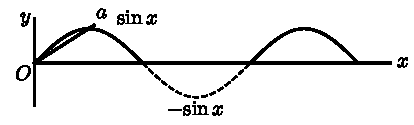
\includegraphics[width=4.5cm]{fig9.pdf}\\[0.3em]{\small 图 9}\end{minipage}\par\nopagebreak

势阱半径 $a$ 愈小，$U_{0,\min}$ 就愈大.第一个能级 $E_1$ 开始出现时所在的位置由 $ka=\frac{1}{2}\pi$ 确定，此时 $E_1=0$.当阱深进一步增加时，基态能级 $E_1$ 下降.当差值 $\Delta=(U_0/U_{0,\min})-1$ 很小时，有
\begin{equation}
  -E_1=(\pi^2/16)U_{0,\min}\Delta^2
\end{equation}

\noindent{\heiti 习题2}\quad 试求：在一个很深的球势阱中（$U_0\gg\hbar^2/ma^2$），角动量 $l$ 值不同的各个能级的排列次序（W. Elsasser,1933）.

解：当 $U_0\to\infty$ 时，阱边的条件要求 $\psi$ 趋于零（参考§22）.把阱内的径向波函数写成(33.10)的形式，可得下列方程
\begin{equation*}
  \mathrm{J}_{l+\frac{1}{2}}(ka)=0,
\end{equation*}
当 $l$ 取不同值时上式的各个根就确定了阱底以上各能级的位置（$\hbar^2k^2/2m=U_0-|E|$）.从基态开始它们的排列次序如下：
\begin{equation*}
  1\mathrm{s},1\mathrm{p},1\mathrm{d},2\mathrm{s},1\mathrm{f},2\mathrm{p},
  1\mathrm{g},2\mathrm{d},1\mathrm{h},3\mathrm{s},2\mathrm{f},\cdots.
\end{equation*}
字母前的数字标志 $l$ 值相同的能级的出现次序\footnote{这种记号对原子核中的粒子能级讲来经常采用（见§118）.}.

\noindent{\heiti 习题3}\quad 试求：当阱深 $U_0$ 逐渐增加时，不同 $l$ 值的各种能级的先后出现次序.

解：每当一个新能级开始出现时，它的能量 $E=0$.此时的阱外波函数为 $R_l=\text{常数}\times r^{-(l+1)}$，满足 $r\to\infty$ 时 $R_l\to0$ 的条件［方程式(33.3)当 $k=0$ 时之解］.根据阱边上 $R_l$ 和 $R'_l$ 的连续性，特别是微商 $(r^{l+1}R_l)'$ 的连续性，可得阱内波函数在这种情形下所满足的条件：
\begin{equation*}
  r=a\ \text{时，}\ (r^{l+1}R_l)'=0,
\end{equation*}
这个条件等价\footnote{按(33.7)(33.8)式，我们有 $(r^{-l}R_l)'=r^{-l}R_{l+1}$. 由于 $l$ 换成 $-l-1$ 时方程式(33.3)保持不变，我们就有 $(r^{l+1}R_{-l-1})'=r^{l+1}R_{-l}$. 最后，由于 $R_{-l}$ 和 $R_{l-1}$ 满足同一方程，从而得
\begin{equation*}
  (r^{l+1}R_l)'=r^{l+1}R_{l-1}
\end{equation*}
这就是题中所用的式子.}于 $r=a$ 时的 $R_{l-1}=0$，再按(33.10)式，得下列方程
\begin{equation*}
  \mathrm{J}_{l-\frac{1}{2}}\left(\frac{a}{\hbar}\sqrt{2mU_0}\right)=0;
\end{equation*}
$l=0$ 时，$\mathrm{J}_{l-\frac{1}{2}}$ 函数应换成余弦函数.由上式可得 $U_0$ 逐渐增大时各个新能级的先后出现次序，如下所示：
\begin{equation*}
  1\mathrm{s},1\mathrm{p},1\mathrm{d},2\mathrm{s},1\mathrm{f},2\mathrm{p},
  1\mathrm{g},2\mathrm{d},3\mathrm{s},1\mathrm{h},2\mathrm{f},\cdots.
\end{equation*}
注意，它和深阱中能级排列次序的差别，仅出现在相当高的能级中.

\noindent{\heiti 习题4}\quad 求一空间振子（势场 $U=\frac{1}{2}m\omega^2r^2$ 中的一个粒子）的能级，并求它的简并度，以及相应定态中轨道角动量的各种可能值.

解：在 $U=\frac{1}{2}m\omega^2(x^2+y^2+z^2)$ 势场中的单粒子薛定谔方程，能用分离变量法归结为三个线性振子方程.故其能级为
\begin{equation*}
  E=\hbar\omega\left(n_1+n_2+n_3+\frac{3}{2}\right)
  =\hbar\omega\left(n+\frac{3}{2}\right).
\end{equation*}
第 $n$ 个能级的简并度，等于把 $n$ 分割成三个正整数（包括零）之和时各种不同分割方法的总数\footnote{换句话说，这就是把 $n$ 个相同的球分配到三个匣子里有多少种不同的分配方法的总数.}；它等于
\begin{equation*}
  \frac{(n+1)(n+2)}{2}.
\end{equation*}
定态波函数为
\setcounter{equation}{0}%
\begin{equation}
  \psi_{n_1n_2n_3}=\text{常数}\times\mathrm{e}^{-\alpha^2r^2/2}
  \mathrm{H}_{n_1}(\alpha x)\mathrm{H}_{n_2}(\alpha y)\mathrm{H}_{n_3}(\alpha z),
\end{equation}
其中的 $\alpha=\sqrt{m\omega/\hbar}$（$m$ 为该粒子质量）.当坐标反号时，$\mathrm{H}_n$ 多项式变成 $(-1)^n\mathrm{H}_n$，故函数(1)的宇称为 $(-1)^{n_1+n_2+n_3}=(-1)^n$.把满足 $n_1+n_2+n_3=n$（$n$ 为给定）的各个 $\psi_{n_1n_2n_3}$ 函数加以线性组合后，可以组成以下一套函数；
\begin{equation}
  \psi_{nlm}=\text{常数}\times\mathrm{e}^{-\alpha^2r^2/2}\,r^l\,
  \mathrm{Y}_{lm}(\theta,\varphi)\,
  \mathrm{F}\left(-\frac{1}{2}n+\frac{1}{2}l,\,l+\frac{3}{2},\,\alpha^2r^2\right),
\end{equation}
其中的 $|m|=0,1,\cdots,l$，而 $l$ 当 $n$ 为偶数时可取 $0,2,\cdots,n$ 诸值，当 $n$ 为奇数时可取 $1,3,\cdots,n$ 诸值.这是由于函数组(1)的宇称为 $(-1)^n$，而函数组(2)的宇称为 $(-1)^l$，这两个宇称必须相同.这就确定了所考虑能级中轨道角动量所能采取的各种可能值.

因此，空间振子的能级次序（采用题2题3中所用的记号）如下：
\begin{equation*}
  (1\mathrm{s}),(1\mathrm{p}),(1\mathrm{d},2\mathrm{s}),
  (1\mathrm{f},2\mathrm{p}),(1\mathrm{g},2\mathrm{d},3\mathrm{s}),\cdots.
\end{equation*}
括号中包括了同一能级的各种简并态\footnote{注意角动量 $l$ 值不同的能级相互简并；见§36 末段的附注.}.

\end{xiti}
\renewcommand{\theequation}{\arabic{section}.\arabic{equation}}%

\section{平面波的分解}

考虑一个自由粒子，沿 $z$ 轴的正方向以给定的动量值 $p=k\hbar$ 运动.这种粒子的波函数呈以下形式：
\begin{equation*}
  \psi=\text{常数}\times\mathrm{e}^{ikz}.
\end{equation*}
\emergencystretch=2em%
我们来把这个函数按自由运动的角动量本征函数 $\psi_{klm}$ 展开.由于所考虑的态中能量具有定值 $k^2\hbar^2/2m$，显然，欲求的展开式中只能出现具有上述 $k$ 值的各种函数.此外，由于 $\mathrm{e}^{ikz}$ 函数对 $z$ 轴具有轴对称性，它的展开式中只能包含与 $\varphi$ 角无关的函数，即 $m=0$ 的各种函数.因此一定有
\begin{equation*}
  \mathrm{e}^{ikz}=\sum_{l=0}^{\infty}a_l\psi_{kl0}
  =\sum_{l=0}^{\infty}a_lR_{kl}\mathrm{Y}_{l0}
\end{equation*}
\emergencystretch=0pt%
其中的 $a_l$ 是一些常数.把(28.8)和(33.9)式的 $\mathrm{Y}_{l0}$ 和 $R_{kl}$ 函数代入上式，我们得
\begin{equation*}
  \mathrm{e}^{ikz}=\sum_{l=0}^{\infty}C_l\mathrm{P}_l(\cos\theta)
  \left(\frac{r}{k}\right)^l\left(\frac{1}{r}\frac{\mathrm{d}}{\mathrm{d}r}\right)^l
  \frac{\sin kr}{kr},\qquad(z=r\cos\theta).
\end{equation*}
其中的 $C_l$ 是另一些常数.上式两边都展成 $r$ 的幂级数后，再比较 $(r\cos\theta)^n$ 前面的系数，就可以把这些常数求出来.对上式的右边讲来，$(r\cos\theta)^n$ 只包含在第 $n$ 个求和项中；因为 $l>n$ 时，径函数的展式是从 $r$ 的更高幂次开始的，而当 $l<n$ 时，$\mathrm{P}_l(\cos\theta)$ 多项式中只含 $\cos\theta$ 的较低次幂.$\mathrm{P}_l(\cos\theta)$ 中 $\cos^l\theta$ 一项的系数为 $(2l)!/2^l(l!)^2$［见(c.1)式］.再用(33.13)式，可得上式右边展开式中的欲求项为
\begin{equation*}
  (-1)^lC_l\frac{(2l)!\,(kr\cos\theta)^l}{2^l(l!)^2(2l+1)!!}
\end{equation*}
上式左边（在 $\mathrm{e}^{ikr\cos\theta}$ 的展开式中）的对应项为
\begin{equation*}
  \frac{(ikr\cos\theta)^l}{l!}.
\end{equation*}
以上两项相等，我们求得 $C_l=(-i)^l(2l+1)$.因此最后求得的展开式为
\begin{equation}
  \mathrm{e}^{ikz}=\sum_{l=0}^{\infty}(-i)^l(2l+1)\mathrm{P}_l(\cos\theta)
  \left(\frac{r}{k}\right)^l\left(\frac{1}{r}\frac{\mathrm{d}}{\mathrm{d}r}\right)^l
  \frac{\sin kr}{kr}.
\end{equation}
此式在远距离处呈下列渐近形式：
\begin{equation}
  \mathrm{e}^{ikz}\approx\frac{1}{kr}\sum_{l=0}^{\infty}i^l(2l+1)
  \mathrm{P}_l(\cos\theta)\sin\left(kr-\frac{1}{2}l\pi\right).
\end{equation}
在(34.1)式中，$z$ 轴是选定在沿着平面波波矢 $\boldsymbol{k}$ 的方向的.这个表式可以写成更一般的形式，使它与坐标轴的选取无关.为此必须应用球谐函数相加定理［见(c.11)］，用 $\boldsymbol{k}$ 方向和 $\boldsymbol{r}$ 方向（两者的夹角为 $\theta$）的球谐函数表出多项式 $\mathrm{P}_l(\cos\theta)$.结果为
\begin{equation}
  \mathrm{e}^{i\boldsymbol{k}\cdot\boldsymbol{r}}=4\pi\sum_{l=0}^{\infty}\sum_{m=-l}^{l}
  i^lj_l(kr)\,\mathrm{Y}^*_{lm}\left(\frac{\boldsymbol{k}}{k}\right)
  \mathrm{Y}_{lm}\left(\frac{\boldsymbol{r}}{r}\right).
\end{equation}
$j_l(kr)$ 函数［由(33.11)式定义］只依赖于乘积 $kr$，使得上式明显地对称于矢量 $\boldsymbol{k}$ 和 $\boldsymbol{r}$；两个球谐函数中，不论哪个取复共轭都毫无关系.

我们把 $\mathrm{e}^{ikz}$ 归一化成概率流密度等于1的波函数，使它对应于这样一股粒子流，该粒子流平行于 $z$ 轴，每单位时间内有一个粒子穿过一个单位面积.这样的归一化波函数为
\begin{equation}
  \psi=\frac{1}{\sqrt{v}}\,\mathrm{e}^{ikz}
  =\sqrt{\frac{m}{k\hbar}}\,\mathrm{e}^{ikz},
\end{equation}
\emergencystretch=2em%
其中 $v$ 为该粒子的速度；见(19.7).(34.1)式两边各乘 $\sqrt{m/k\hbar}$ 并在式右引进归一化的 $\psi^{\pm}_{klm}=R^{\pm}_{kl}(r)\mathrm{Y}_{lm}(\theta,\varphi)$ 函数后，我们得
\begin{equation*}
  \psi=\sum_{l=0}^{\infty}\sqrt{\pi(2l+1)}\,\frac{i^l}{ik}
  \left(\psi^+_{kl0}-\psi^-_{kl0}\right).
\end{equation*}
\emergencystretch=0pt%
按照一般规则，这个展开式中 $\psi^-_{kl0}$（或 $\psi^+_{kl0}$）前面的系数的模量平方值，等于汇于原点（或从原点发出）的粒子流中一个粒子具有角动量 $l$（相对于原点）的概率.由于波函数 $v^{-1/2}\mathrm{e}^{ikz}$ 相当于流密度为1的粒子流，这个“概率”就具有面积的量纲；它可以直观地解释成角动量为 $l$ 的粒子所应通过的那个“截面”（在 $xy$ 平面内）的面积.用 $\sigma_l$ 代表这个量，我们有
\begin{equation}
  \sigma_l=\frac{\pi}{k^2}(2l+1).
\end{equation}
$l$ 值很大时，在 $\Delta l$ 区间内（此时有 $1\ll\Delta l\ll l$）的截面之和等于
\begin{equation*}
  \sum_{\Delta l}\sigma_l\approx\frac{\pi}{k^2}2l\Delta l
  =2\pi\frac{l\hbar^2}{p^2}\Delta l.
\end{equation*}
把角动量的经典表式 $\hbar l=\rho p$ 代入（$\rho$ 称为碰撞参量），上式变成
\begin{equation*}
  2\pi\rho\Delta\rho,
\end{equation*}
就与经典结果相一致.这样的结果并不是偶然的；以后将看到，$l$ 值很大时，运动是准经典的（见§49）.

\begin{xiti}

\noindent{\heiti 习题}\quad 试将一个平面波按照一组态的波函数展开，这组态在 $y$ 轴上具有确定的角动量分量 $m$ 和动量分量 $p_y$.

解：引入其轴与 $y$ 轴一致的柱面坐标系 $y,\rho,\varphi$.题中所给的那些态的波函数将具有下列形式：
\begin{equation*}
  Q_m(\rho)\,\mathrm{e}^{im\varphi}\,\mathrm{e}^{ip_yy/\hbar}
\end{equation*}
取 $\varphi$ 为径矢与 $z$ 轴所成的角度，则展开式为
\begin{equation*}
  \mathrm{e}^{ikz}=\mathrm{e}^{ik\rho\cos\varphi}
  =\sum_{m=-\infty}^{\infty}Q_m(\rho)\,\mathrm{e}^{im\varphi}
\end{equation*}
（此时 $p_y=0$），由此得
\begin{equation*}
  Q_m(\rho)=\frac{1}{2\pi}\int_0^{2\pi}
  \exp\left[i(k\rho\cos\varphi-m\varphi)\right]\mathrm{d}\varphi
  =i^m\mathrm{J}_m(k\rho),
\end{equation*}
式中 $\mathrm{J}_m(x)$ 为贝塞尔函数.当 $k\rho\gg1$ 时 $Q_m$ 的渐近形式为
\begin{equation*}
  Q_m(\rho)\approx i^m\sqrt{\frac{2}{\pi k\rho}}\,
  \sin\left[k\rho-\frac{\pi}{2}\left(m-\frac{1}{2}\right)\right].
\end{equation*}

\end{xiti}

\section{粒子向力心的“坠落”}

为了揭示量子力学运动的某些特性，我们来考察一种有益的情况，尽管这种情况本身并没有直接的物理意义：设有一粒子运动于某一势场中，该场在某点（原点）按 $U(r)\approx-\beta/r^2$（$\beta>0$）的规律趋向无穷大；场在远离原点处的形状，我们不予考虑.我们在§18中已经看到，这样的情况，是介于通常的定态运动和粒子向力心的“坠落”这两种情况之间的.

在原点附近，薛定谔方程现在变成
\begin{equation}
  R''+\frac{2}{r}R'+\frac{\gamma}{r^2}R=0
\end{equation}
［$R(r)$ 为波函数的径部］，式中引进了下列常数：
\begin{equation}
  \gamma=\frac{2m\beta}{\hbar^2}-l(l+1),
\end{equation}
并且已经略去了幂次低于 $1/r$ 的所有各项；能量 $E$ 的数值假定是有限的，因而含 $E$ 之项亦已在方程中略去.

我们假定 $R$ 的形状为 $R\sim r^s$；则可得出 $s$ 的一个二次方程：
\begin{equation*}
  s(s+1)+\gamma=0,
\end{equation*}
它有以下两个根：
\begin{equation}
  s_1=-\frac{1}{2}+\sqrt{\frac{1}{4}-\gamma},\qquad
  s_2=-\frac{1}{2}-\sqrt{\frac{1}{4}-\gamma}.
\end{equation}
为了进一步研究这个问题，最好采用以下的步骤.我们先绕原点划出一个半径为 $r_0$ 的小区域，并用常数 $-\gamma/r_0^2$ 代替这个区域内的 $-\gamma/r^2$ 函数.然后把这个“被截断的”场中的波函数求出来，再来研究过渡到极限情形 $r_0\to0$ 时能得什么结果.

我们先假定 $\gamma<\frac{1}{4}$.此时 $s_1$ 和 $s_2$ 都是负实数，并且 $s_1>s_2$，对 $r>r_0$ 而言，薛定谔方程的通解具有下列形式（我们永远限于 $r$ 很小时的情形）：
\begin{equation}
  R=Ar^{s_1}+Br^{s_2},
\end{equation}
$A$ 和 $B$ 都是常数.当 $r<r_0$ 时，方程
\begin{equation*}
  R''+\frac{2}{r}R'+\frac{\gamma}{r_0^2}R=0
\end{equation*}
的解如果在原点取有限值，则此解的形式为
\begin{equation}
  R=C\frac{\sin kr}{r},\qquad k=\frac{\sqrt{\gamma}}{r_0}.
\end{equation}
$r=r_0$ 处，$R$ 函数及其导数 $R'$ 必须连续.这两个连续条件最好改为一个条件，$rR$ 的对数导数为连续.由此得出下列式子：
\begin{equation*}
  \frac{A(s_1+1)r_0^{s_1}+B(s_2+1)r_0^{s_2}}
  {Ar_0^{s_1+1}+Br_0^{s_2+1}}=k\cot kr_0
\end{equation*}
或
\begin{equation*}
  \frac{A(s_1+1)r_0^{s_1}+B(s_2+1)r_0^{s_2}}
  {Ar_0^{s_1}+Br_0^{s_2}}=\sqrt{\gamma}\cot\sqrt{\gamma}.
\end{equation*}
从上式解出的比值 $B/A$ 呈以下的形式：
\begin{equation}
  \frac{B}{A}=\text{常数}\times r_0^{s_1-s_2}.
\end{equation}
现在让 $r_0\to0$，我们发现 $B/A\to0$（注意 $s_1>s_2$）.由此可见，对薛定谔方程(35.1)的两个在原点处发散的解讲来，我们应该选取发散得较慢的那个解：
\begin{equation}
  R=\frac{A}{r^{-s_1}}.
\end{equation}
现在设 $\gamma>\frac{1}{4}$.此时 $s_1$ 和 $s_2$ 都成为复数：
\begin{equation*}
  s_1=-\frac{1}{2}+i\sqrt{\gamma-\frac{1}{4}},\qquad s_2=s_1^*.
\end{equation*}
重复以上的分析，结果仍得(35.6)式，把 $s_1$ 和 $s_2$ 的值代入以后得到
\begin{equation}
  \frac{B}{A}=\text{常数}\times r_0^{i\sqrt{4\gamma-1}}.
\end{equation}
过渡到极限情形 $r_0\to0$ 时，上式并不趋向任何固定的极限值，可见不可能直接过渡到极限.采用(35.8)式，则实解的一般形式可以写成
\begin{equation}
  R=\text{常数}\times r^{-\frac{1}{2}}
  \cos\left(\sqrt{\gamma-\frac{1}{4}}\ln\frac{r}{r_0}+\text{常数}\right).
\end{equation}
这个函数所具的零点数随 $r_0$ 的减小而无限增多.一方面，由于(35.9)式对具有任意有限能量值 $E$ 的波函数（指 $r$ 很小时的波函数）讲来都能成立，另一方面，基态波函数是根本没有零点的，我们就可以得出这样的推论，该场中粒子的“基态”对应于能量 $E=-\infty$.对离散谱的任一状态讲来，粒子主要是在 $E>U$ 的空间区域内.因此，当 $E\to-\infty$ 时，该粒子处在原点附近的无限小区域内，这就是说，该粒子“落”入力心.

粒子开始“落”入力心的“临界”场 $U_{cr}$ 相当于 $\gamma=\frac{1}{4}$.$U_{cr}$ 中 $-1/r^2$ 前面的最小系数可以从 $l=0$ 的(35.2)式得出，即
\begin{equation}
  U_{cr}=-\frac{\hbar^2}{8mr^2}.
\end{equation}
由(35.3)式（式中的 $s_1$）可以看出，薛定谔方程允许解（在 $U\sim1/r^2$ 的附近）的发散程度在 $r\to0$ 时不快于 $1/\sqrt{r}$.如果 $r\to0$ 时该势场比 $1/r^2$ 更慢地趋向无穷大，则在原点附近的薛定谔方程中，$U(r)$ 与其它项相比可以略去不计，从而得到和自由运动相同的解，即 $\psi\sim r^l$（见§33）.最后，如果势场比 $1/r^2$ 更快地趋向无穷大（按 $-1/r^s$ 规律，$s>2$），那么，原点附近的波函数就和 $r^{s/4-1}$ 成正比（见§49例题）.在所有以上情况下，乘积 $r\psi$ 在 $r=0$ 点都趋于零.

其次，我们来研究场在无穷远处按 $U\approx-\beta/r^2$ 的规律消失并在原点附近具有任意形式时，薛定谔方程之解所具有的性质.我们首先假定 $\gamma<\frac{1}{4}$.容易证明这种情形下只能存在有限多个负能级\footnote{这里已经假定了 $r$ 很小时该场中的粒子不会“落”入力心.}.实际上，能量 $E=0$ 时，薛定谔方程在远距离处呈(35.1)形式，它的通解为(35.4)式.可是(35.4)式的函数是没有零点的（$r\neq0$ 时）；因此，径向波函数的所有零点都位于有限距离内，它们的总数是有限的.换句话说，离散谱的终止能级 $E=0$ 的编号是一个有限值.

另一方面，如果 $\gamma>\frac{1}{4}$，离散谱就含无穷多个负能级.实际上，$E=0$ 的状态波函数在远距离处呈(35.9)形式，具有无穷多个零点，从而其编号永远是无穷大.

最后，设场在整个空间内呈 $U=-\beta/r^2$ 形式.如果 $\gamma>\frac{1}{4}$，该粒子就“落”入力心，如果 $\gamma<\frac{1}{4}$，则完全不存在负能级.实际上，此时 $E=0$ 的状态其波函数在整个空间内呈(35.7)形式；这个式子，在有限距离内没有零点，亦即它对应于最低的能级（对给定的 $l$ 而言）.

\section{库仑场中的运动（球坐标）}

有心力场运动中一个极重要的情形是库仑场
\begin{equation*}
  U=\pm\alpha/r
\end{equation*}
中的运动（其中 $\alpha$ 是一个正的常数）.我们先考虑库仑引力场，因而写成 $U=-\alpha/r$.根据以前讲过的一般考虑，显然负能量本征值呈离散谱（具有无穷多个能级），正能量本征值呈连续谱.

(32.8)的径函数方程呈以下形式：
\begin{equation}
  \frac{\mathrm{d}^2R}{\mathrm{d}r^2}+\frac{2}{r}\frac{\mathrm{d}R}{\mathrm{d}r}
  -\frac{l(l+1)}{r^2}R+\frac{2m}{\hbar^2}\left(E+\frac{\alpha}{r}\right)R=0.
\end{equation}
如果我们考虑的是两个相吸粒子的相对运动，$m$ 应取折合质量.

在涉及库仑场的计算中，最好采用一种特殊的单位制代替通常的单位制，我们称它为库仑单位制.这种单位制中的质量、长度和时间的量度单位分别为
\begin{equation*}
  m,\qquad\frac{\hbar^2}{m\alpha},\qquad\frac{\hbar^3}{m\alpha^2}.
\end{equation*}
所有其它单位都可以从以上三个单位导出；例如能量的单位为
\begin{equation*}
  \frac{m\alpha^2}{\hbar^2}.
\end{equation*}
在本节及下节中，我们都采用这种单位制（除非作特殊声明）\footnote{如令 $m=9.11\times10^{-31}\,\mathrm{kg}$ 为电子的质量，并令 $\alpha=e^2$（$e$ 为电子的电荷），则库仑单位制就和\textbf{原子单位制}一致. 长度的原子单位为
\begin{equation*}
  \hbar^2/me^2=0.529\times10^{-10}\ \mathrm{m}
\end{equation*}
（称为玻尔半径）. 能量的原子单位为
\begin{equation*}
  me^4/\hbar^2=4.36\times10^{-18}\ \mathrm{J}=27.21\ \mathrm{eV}.
\end{equation*}
取这个单位的一半，称为 1 里德伯（rydberg）. 电荷的原子单位为 $e=1.60\times10^{-19}\ \mathrm{C}$. 在原式中形式地令 $e=m=\hbar=1$，我们就得到原子单位制中的各个公式. 对于 $\alpha=Ze^2$，库仑单位就和原子单位不同.}.

(36.1)式在新单位制中变成
\begin{equation}
  \frac{\mathrm{d}^2R}{\mathrm{d}r^2}+\frac{2}{r}\frac{\mathrm{d}R}{\mathrm{d}r}
  -\frac{l(l+1)}{r^2}R+2\left(E+\frac{1}{r}\right)R=0.
\end{equation}

\subsection*{离散谱}

引入下列新量代替参量 $E$ 和变量 $r$：
\begin{equation}
  n=\frac{1}{\sqrt{-2E}},\qquad\rho=\frac{2r}{n}.
\end{equation}
$E$ 为负值时，$n$ 是一个正实数.(36.2)式作(36.3)式的替代后呈下列形式：
\begin{equation}
  R''+\frac{2}{\rho}R'
  +\left[-\frac{1}{4}+\frac{n}{\rho}-\frac{l(l+1)}{\rho^2}\right]R=0
\end{equation}
（撇号代表对 $\rho$ 取微商）.

$\rho$ 很小时，满足有限性条件之解与 $\rho^l$ 成正比［见(32.15)式］.$\rho$ 很大时，要计算 $R$ 的渐近行为，我们可在(36.4)式中略去含有 $1/\rho$ 和 $1/\rho^2$ 的项，得下列方程：
\begin{equation*}
  R''=\frac{1}{4}R,
\end{equation*}
故 $R=\mathrm{e}^{\pm\frac{1}{2}\rho}$.我们只对无穷远处等于零的解感兴趣，可见，$\rho$ 很大时，这个解应按 $\mathrm{e}^{-\frac{1}{2}\rho}$ 的规律递减.

据此我们很自然地作下列替代：
\begin{equation}
  R=\rho^l\mathrm{e}^{-\frac{1}{2}\rho}\,w(\rho),
\end{equation}
此时，(36.4)式变成
\begin{equation}
  \rho w''+(2l+2-\rho)w'+(n-l-1)w=0.
\end{equation}
此式之解在无穷远处应该不比 $\rho$ 的任意有限次幂发散得更快，而当 $\rho=0$ 时应该等于一个有限值.满足后一条件的解为下列合流超几何函数：
\begin{equation}
  w=\mathrm{F}(-n+l+1,2l+2,\rho)
\end{equation}
（见数学附录§d）\footnote{(36.6)式的第二种解当 $\rho\to0$ 时按 $\rho^{-2l-1}$ 方式发散.}.满足无穷远处条件之解，要求(36.7)式中的 $-n+l+1$ 只能取负整数（或零），此时，(36.7)式所示的函数变成一个 $\rho$ 的 $n-l-1$ 次多项式.否则(36.7)式在无穷远处将按 $\mathrm{e}^{\rho}$ 方式发散［见(d.14)式］.

由此得出结论，$n$ 必须是一个正整数，对给定的 $l$ 而言，必须有
\begin{equation}
  n\geqslant l+1.
\end{equation}
忆及(36.3)式中参量 $n$ 的定义，我们得到
\begin{equation}
  E=-\frac{1}{2n^2},\qquad n=1,2,\cdots.
\end{equation}
这就解决了库仑场中离散谱的能级问题.我们看到，在零与基态能级 $E_1=-\frac{1}{2}$ 之间，存在着无穷多个能级.相邻能级的间距随 $n$ 的增大而递减；这些能级愈来愈密地挤向 $E=0$ 的能级，在 $E=0$ 处，离散谱宣告终止而转为连续谱.在通常的单位制中，(36.9)式呈下列形式\footnote{在量子力学出现之前的 1913 年，N.~玻尔首先得到(36.10)式. 量子力学中，泡利于 1926 年运用矩阵方法得到此式，几个月后，薛定谔（运用波动方程）又求出此式.}：
\begin{equation}
  E=-\frac{m\alpha^2}{2\hbar^2n^2}.
\end{equation}
整数 $n$ 称为主量子数.§32 中定义的径量子数等于
\begin{equation*}
  n_r=n-l-1.
\end{equation*}
主量子数的数值给定后，$l$ 可取以下各种数值：
\begin{equation}
  l=0,1,\cdots,n-1,
\end{equation}
即 $l$ 可取 $n$ 个不同的数值.(36.9)的能量表式中只出现 $n$.因此，$n$ 相同 $l$ 不同的各种态具有相同的能量值.由此可见，每一个本征值，不但对磁量子数 $m$ 而言（这是任意有心力场所共有的）而且对 $l$ 而言都是简并的.后一种简并（称为偶然简并或库仑简并）是库仑场特有的性质.我们知道，对每一个 $l$ 值而言，有 $(2l+1)$ 个不同的 $m$ 值.因此第 $n$ 个能级的简并度等于
\begin{equation}
  \sum_{l=0}^{n-1}(2l+1)=n^2.
\end{equation}
定态波函数是由(36.5)和(36.7)式确定的.合流超几何函数的两个参量都为整数时，除开一个因子外，等于广义拉盖尔函数（见数学附录§d），故
\begin{equation*}
  R_{nl}=\text{常数}\times\rho^l\mathrm{e}^{-\frac{1}{2}\rho}\,
  \mathrm{L}_{n+l}^{2l+1}(\rho).
\end{equation*}
径函数应按下列条件归一化：
\begin{equation*}
  \int_0^{\infty}R_{nl}^2r^2\,\mathrm{d}r=1.
\end{equation*}
其最终形式为\footnote{我们给出前面几个 $R_{nl}$ 函数：
\begin{equation*}
\begin{gathered}
  R_{10}=2\mathrm{e}^{-r},\qquad
  R_{20}=\frac{1}{\sqrt{2}}\,\mathrm{e}^{-\frac{1}{2}r}
  \left(1-\frac{1}{2}r\right),\qquad
  R_{21}=\frac{1}{2\sqrt{6}}\,\mathrm{e}^{-\frac{1}{2}r}r,\\
  R_{30}=\frac{2}{3\sqrt{3}}\,\mathrm{e}^{-\frac{1}{3}r}
  \left(1-\frac{2}{3}r+\frac{2}{27}r^2\right),\\
  R_{31}=\frac{8}{27\sqrt{6}}\,\mathrm{e}^{-\frac{1}{3}r}\,
  r\left(1-\frac{r}{6}\right),\qquad
  R_{32}=\frac{4}{81\sqrt{30}}\,\mathrm{e}^{-\frac{1}{3}r}\,r^2
\end{gathered}
\end{equation*}}
\begin{equation}
\begin{aligned}
  R_{nl}={}&-\frac{2}{n^2}\sqrt{\frac{(n-l-1)!}{\left[(n+l)!\right]^3}}\,
  \mathrm{e}^{-r/n}\left(\frac{2r}{n}\right)^l\mathrm{L}_{n+l}^{2l+1}\left(\frac{2r}{n}\right)=\\
  ={}&\frac{2}{n^{l+2}(2l+1)!}\sqrt{\frac{(n+l)!}{(n-l-1)!}}\,\times\\
  &\times(2r)^l\,\mathrm{e}^{-r/n}\,
  \mathrm{F}\left(-n+l+1,2l+2,\frac{2r}{n}\right)
\end{aligned}
\end{equation}
这个归一化积分是用(f.6)式算出的\footnote{把拉盖尔多项式的表式(d.13)代入，并进行分部积分，也能算出这个归一化积分［与计算勒让德多项式的积分式(c.8)相似］.}.

在原点附近，$R_{nl}$ 呈下列形式：
\begin{equation}
  R_{nl}\approx r^l\frac{2^{l+1}}{n^{2+l}(2l+1)!}
  \sqrt{\frac{(n+l)!}{(n-l-1)!}}.
\end{equation}
在远距离处，
\begin{equation}
  R_{nl}\approx(-1)^{n-l-1}
  \frac{2^n}{n^{n+1}\sqrt{\left[(n+l)!\,(n-l-1)!\right]}}\,
  r^{n-1}\mathrm{e}^{-r/n}
\end{equation}
当距离 $r$ 的数量级达到 $r\sim1$ 时（在通常单位制中 $r\sim\hbar^2/m\alpha$ 时），基态波函数 $R_{10}$ 指数式地下降.

$r$ 的各种幂次的平均值是用下式计算的：
\begin{equation*}
  \overline{r^k}=\int_0^{\infty}r^{k+2}R_{nl}^2\,\mathrm{d}r.
\end{equation*}
应用(f.7)式可以求得 $\overline{r^k}$ 的通式.我们在这里写出前几个 $\overline{r^k}$ 值（包括正、负 $k$ 值）：
\begin{equation}
\begin{gathered}
  \overline{r}=\frac{1}{2}\left[3n^2-l(l+1)\right],\qquad
  \overline{r^2}=\frac{1}{2}n^2\left[5n^2+1-3l(l+1)\right],\\
  \overline{r^{-1}}=\frac{1}{n^2},\qquad
  \overline{r^{-2}}=\frac{1}{n^3(l+1/2)}.
\end{gathered}
\end{equation}

\subsection*{连续谱}

正能量本征值呈连续谱，从零一直延伸到无穷大.每一个这样的本征值都是无穷简并的；因为每一个 $E$ 值有无穷多个态与之对应，这些态中的 $l$，可取零到 $\infty$ 的所有整数值（对给定的 $l$ 而言，$m$ 还可取各种可能的数值）.

(36.3)式中定义的数值 $n$ 及变量 $\rho$，现在都变成纯虚量：
\begin{equation}
  n=-\frac{i}{\sqrt{2E}}=-\frac{i}{k},\qquad\rho=2ikr,
\end{equation}
其中 $k=\sqrt{2E}$\footnote{$n$ 和 $\rho$ 也可以用复共轭表式 $n=i/k,\rho=-2ikr$ 定义；实函数 $R_{kl}$ 当然与采用哪一种定义无关.}.连续谱的径函数呈下列形式：
\begin{equation}
  R_{kl}=\frac{C_{kl}}{(2l+1)!}(2kr)^l\mathrm{e}^{-ikr}
  \mathrm{F}\left(\frac{i}{k}+l+1,2l+2,2ikr\right),
\end{equation}
其中的 $C_{kl}$ 是归一化因子.这些径函数可以表成下列复积分形式（见§d）：
\begin{equation}
  R_{kl}=C_{kl}(2kr)^l\mathrm{e}^{-ikr}\frac{1}{2\pi i}
  \oint\mathrm{e}^{\xi}\left(1-\frac{2ikr}{\xi}\right)^{-\frac{i}{k}-l-1}
  \xi^{-2l-2}\,\mathrm{d}\xi,
\end{equation}
所取的积分路线\footnote{我们也可以用沿正方向绕过 $\xi=0$ 和 $\xi=2ikr$ 两个奇点的任意一条封闭曲线来代替图 10 中的积分曲线. 对整数的 $l$，函数 $V(\xi)=\xi^{-n-l}(\xi-2ikr)^{n-l}$（见§d）绕此曲线一周回到原值.}如图10所示.通过替代 $\xi=2ikr\left(t+\frac{1}{2}\right)$，这个积分可以化成更为对称的形式：
\begin{equation}
  R_{kl}=C_{kl}\frac{(-2kr)^{-l-1}}{2\pi}
  \oint\mathrm{e}^{2iktr}\left(t+\frac{1}{2}\right)^{\frac{i}{k}-l-1}
  \left(t-\frac{1}{2}\right)^{-\frac{i}{k}-l-1}\mathrm{d}t,
\end{equation}
所取的积分路线沿正方向绕过 $t=\pm\frac{1}{2}$ 两点.根据这个表式立刻可以看出函数 $R_{kl}$ 都是实函数.

\par\nopagebreak\noindent\begin{minipage}{\linewidth}\centering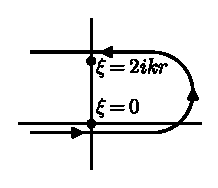
\includegraphics[width=4cm]{fig10.pdf}\\[0.3em]{\small 图 10}\end{minipage}\par\nopagebreak

利用合流超几何函数(d.14)的渐近展式，可以立刻求得波函数 $R_{kl}$ 的类似展式.(d.14)式中的两项给出了函数 $R_{kl}$ 中的两个复共轭表式，结果得
\begin{equation}
\begin{aligned}
  R_{kl}=C_{kl}\frac{\mathrm{e}^{-\pi/2k}}{kr}\,
  \mathrm{Re}\bigg\{&\frac{\mathrm{e}^{-i\left[kr-\frac{1}{2}\pi(l+1)
  +\left(\frac{1}{k}\right)\ln 2kr\right]}}{\Gamma(l+1-i/k)}\times\\
  &\times\mathrm{G}\left(l+1+\frac{i}{k},\frac{i}{k}-l,-2ikr\right)\bigg\}.
\end{aligned}
\end{equation}
如果波函数按“$k/2\pi$ 标度”归一化［即按条件(33.4)归一化］，则归一化系数等于
\begin{equation}
  C_{kl}=2k\,\mathrm{e}^{\pi/2k}\left|\Gamma\left(l+1-\frac{i}{k}\right)\right|.
\end{equation}
因而当 $r$ 很大时，$R_{kl}$ 的渐近表式［即(36.21)式的展开式中的首项］具有下列形式：
\begin{equation}
\begin{aligned}
  R_{kl}&\approx\frac{2}{r}\sin\left(kr+\frac{1}{k}\ln 2kr-\frac{1}{2}l\pi+\delta_l\right),\\
  \delta_l&=\arg\,\Gamma\left(l+1-\frac{i}{k}\right),
\end{aligned}
\end{equation}
这和有心力场中连续谱的归一化波函数所具有的一般公式(33.20)相一致.(36.23)式和(33.20)式不同之处，在于正弦函数的宗量中存在一个对数项；但由于 $\ln r$ 与 $r$ 相比增长较慢，在计算无穷远处为发散的归一化积分时，这一项的存在是无关紧要的.

出现于归一化因子(36.22)式中的伽马函数的模量值，可以用初等函数表出.应用熟知的伽马函数的性质：
\begin{equation*}
  \Gamma(z+1)=z\Gamma(z),\qquad
  \Gamma(z)\Gamma(1-z)=\frac{\pi}{\sin\pi z},
\end{equation*}
我们有
\begin{equation*}
\begin{aligned}
  \Gamma\left(l+1+\frac{i}{k}\right)&=\left(l+\frac{i}{k}\right)\cdots
  \left(1+\frac{i}{k}\right)\frac{i}{k}\,\Gamma\left(\frac{i}{k}\right),\\
  \Gamma\left(l+1-\frac{i}{k}\right)&=\left(l-\frac{i}{k}\right)\cdots
  \left(1-\frac{i}{k}\right)\Gamma\left(1-\frac{i}{k}\right).
\end{aligned}
\end{equation*}
以及
\begin{equation*}
\begin{aligned}
  \left|\Gamma\left(l+1-\frac{i}{k}\right)\right|&=
  \left[\Gamma\left(l+1-\frac{i}{k}\right)\Gamma\left(l+1+\frac{i}{k}\right)\right]^{1/2}=\\
  &=\sqrt{\frac{\pi}{k}}\prod_{s=1}^{l}\sqrt{s^2+\frac{1}{k^2}}\;
  \sinh^{-\frac{1}{2}}\frac{\pi}{k}.
\end{aligned}
\end{equation*}
故
\begin{equation}
  C_{kl}=\frac{\sqrt{8\pi k}}{\sqrt{1-\mathrm{e}^{-2\pi/k}}}
  \prod_{s=1}^{l}\sqrt{s^2+\frac{1}{k^2}}
\end{equation}
$l=0$ 时，乘积变成1.

取极限 $k\to0$，便能得到零能量特殊情况下的径函数，对此有
\begin{equation*}
\begin{aligned}
  \mathrm{F}\left(\frac{i}{k}+l+1,2l+2,2ikr\right)&\to
  \mathrm{F}\left(\frac{i}{k},2l+2,2ikr\right)=\\
  &=1-\frac{2r}{(2l+2)\cdot 1!}
  +\frac{(2r)^2}{(2l+2)(2l+3)\cdot 2!}-\cdots=\\
  &=(2l+1)!(2r)^{-l-\frac{1}{2}}\mathrm{J}_{2l+1}(\sqrt{8r}),
\end{aligned}
\end{equation*}
其中的 $\mathrm{J}_{2l+1}$ 是 $2l+1$ 阶贝塞尔函数.(36.24)中的 $C_{kl}$ 系数，当 $k\to0$ 时，趋向于
\begin{equation*}
  C_{kl}\approx\sqrt{8\pi}\,k^{-l+\frac{1}{2}}.
\end{equation*}
故
\begin{equation}
  \left.\frac{R_{kl}}{\sqrt{k}}\right|_{k\to0}
  =\sqrt{\frac{4\pi}{r}}\,\mathrm{J}_{2l+1}(\sqrt{8r}),
\end{equation}
$r$ 很大时，这个函数的渐近式为\footnote{注意，这个函数相当于 $\left(l+\frac{1}{2}\right)^2\ll r\ll k^{-2}$ 运动区域内所用的准经典近似式（§49）.}
\begin{equation}
  \left.\frac{R_{kl}}{\sqrt{k}}\right|_{k\to0}
  =\left(\frac{8}{r^3}\right)^{1/4}\sin\left(\sqrt{8r}-l\pi-\frac{\pi}{4}\right).
\end{equation}
如果改为以能量标度归一化，即把 $R_{kl}$ 改成(33.5)式的 $R_{El}$，则上式的 $\sqrt{k}$ 因子消失；$E\to0$ 时，$R_{El}$ 保持有限.

在库仑斥力场中（$U=\alpha/r$）只存在正能量本征值的连续谱.从数学形式上讲来，把库仑引力场方程式中的 $r$ 改成 $-r$，就可得到斥力场中的薛定谔方程.因此，(36.18)式作同一更改后，立刻得到斥力场中的定态波函数.归一化系数仍由渐近表式所确定，所得的结果为
\begin{equation}
\begin{aligned}
  R_{kl}&=\frac{C_{kl}}{(2l+1)!}(2kr)^l\mathrm{e}^{ikr}
  \mathrm{F}\left(\frac{i}{k}+l+1,2l+2,-2ikr\right),\\
  C_{kl}&=2k\,\mathrm{e}^{-\pi/2k}\left|\Gamma\left(l+1+\frac{i}{k}\right)\right|
  =\frac{\sqrt{8\pi k}}{\sqrt{\mathrm{e}^{2\pi/k}-1}}
  \prod_{s=1}^{l}\sqrt{s^2+\frac{1}{k^2}}.
\end{aligned}
\end{equation}
$r$ 很大时这个函数呈下列渐近形式：
\begin{equation}
\begin{aligned}
  R_{kl}&\approx\frac{2}{r}\sin\left(kr-\frac{1}{k}\ln 2kr-\frac{1}{2}l\pi+\delta_l\right),\\
  \delta_l&=\arg\,\Gamma\left(l+1+\frac{i}{k}\right).
\end{aligned}
\end{equation}

\subsection*{库仑简并的本质}

粒子在库仑场中作经典运动时，这种形式的场有一个特殊的守恒定律；如果是引力场，则有（见《力学》§15）
\begin{equation}
  \boldsymbol{A}=\frac{\boldsymbol{r}}{r}-\boldsymbol{p}\times\hat{\boldsymbol{l}}=\text{常数}.
\end{equation}
量子力学中，相应算符为
\begin{equation}
  \hat{\boldsymbol{A}}=\frac{\boldsymbol{r}}{r}
  -\frac{1}{2}\left(\boldsymbol{p}\times\hat{\boldsymbol{l}}
  -\hat{\boldsymbol{l}}\times\boldsymbol{p}\right),
\end{equation}
容易证明，它和哈密顿量 $\hat{H}=\frac{1}{2}\boldsymbol{p}^2-\frac{1}{r}$ 对易.

由直接计算，给出算符 $\hat{A}_i$ 之间以及它和角动量算符之间的下列对易关系：
\begin{equation}
  [\hat{l}_i,\hat{A}_k]=i\mathrm{e}_{ikl}\hat{A}_l,\qquad
  [\hat{A}_i,\hat{A}_k]=-2i\hat{H}\mathrm{e}_{ikl}\hat{l}_l.
\end{equation}
$\hat{A}_i$ 之间的不对易性，说明 $A_x,A_y,A_z$ 三个量在量子力学中不能同时有定值.其中的任一个算符，例如 $\hat{A}_z$，与相应的角动量分量 $\hat{l}_z$ 对易，但和角动量平方算符 $\hat{l}^2$ 不对易.这个附加守恒量的存在，而又不能和其它量同时测量，导致了能级的附加简并（见§10），这就是离散能级的“偶然”简并，为库仑场所特有.

这种简并性的由来，还可以用量子力学库仑问题中与空间旋转对称性相比所增的对称性来加以表述（В.~А.~Фок1935）.为此，我们注意到，具有固定负能量值的离散谱态中，我们可把(36.31)第二式右边的 $\hat{H}$ 改成 $E$，并用算符 $\hat{u}_i=\hat{A}_i/\sqrt{-2E}$ 代替 $\hat{A}_i$.这些算符的对易关系为
\begin{equation}
  [\hat{l}_i,\hat{u}_k]=i\mathrm{e}_{ikl}\hat{u}_l,\qquad
  [\hat{u}_i,\hat{u}_k]=i\mathrm{e}_{ikl}\hat{l}_l.
\end{equation}
上式和对易式 $[\hat{l}_i,\hat{l}_k]=i\mathrm{e}_{ikl}\hat{l}_l$ 放在一起，形式上等同于四维欧氏空间中无限小转动算符的对易关系\footnote{此时 $\hat{l}_x,\hat{l}_y,\hat{l}_z$ 代表四维笛卡儿坐标系 $x,y,z,u$ 中 $yz,zx$ 和 $xy$ 平面内的无限小转动算符；$\hat{u}_x,\hat{u}_y,\hat{u}_z$ 是在 $xu,yu$ 和 $zu$ 平面内的无限小转动算符.}.这就是量子力学中库仑问题的对称性\footnote{在波函数的动量表象中显示的对称性；见 V.~A.~Fok, Zeitschrift für Physik 98, 145, 1935.}.

从对易关系(36.32)出发，我们又能导出库仑场中的能级表式\footnote{这个推导基本上与 W.~泡利（1935）给出的推导相同.}.先把 $\hat{\boldsymbol{l}}$ 和 $\hat{\boldsymbol{u}}$ 改写成下列算符：
\begin{equation}
  \hat{\boldsymbol{j}}_1=\frac{1}{2}\left(\hat{\boldsymbol{l}}+\hat{\boldsymbol{u}}\right),
  \qquad
  \hat{\boldsymbol{j}}_2=\frac{1}{2}\left(\hat{\boldsymbol{l}}-\hat{\boldsymbol{u}}\right).
\end{equation}
对此，有
\begin{equation}
\begin{aligned}
  &[\hat{j}_{1i},\hat{j}_{1k}]=i\mathrm{e}_{ikl}\hat{j}_{1l},\qquad
  [\hat{j}_{2i},\hat{j}_{2k}]=i\mathrm{e}_{ikl}\hat{j}_{2l},\\
  &[\hat{j}_{1i},\hat{j}_{2k}]=0.
\end{aligned}
\end{equation}
上式等同于两个独立的三维角动量矢量的对易关系式.因此 $j_1^2$ 和 $j_2^2$ 的本征值为 $j_1(j_1+1)$ 和 $j_2(j_2+1)$，其中 $j_1,j_2=0,\frac{1}{2},1,\frac{3}{2},\cdots$，\footnote{此处我们提前提到了角动量在 §54 中所描述的性质（$j$ 可以是整数和半整数）.}另一方面，根据算符 $\hat{\boldsymbol{u}}$ 和 $\hat{\boldsymbol{l}}=\boldsymbol{r}\times\hat{\boldsymbol{p}}$ 的定义，经简单计算后，得
\begin{gather*}
  \hat{\boldsymbol{l}}\cdot\hat{\boldsymbol{u}}
  =\hat{\boldsymbol{u}}\cdot\hat{\boldsymbol{l}}=0,\\
  \hat{\boldsymbol{l}}^2+\hat{\boldsymbol{u}}^2=-1-\frac{1}{2E},
\end{gather*}
在 $\hat{\boldsymbol{l}}^2+\hat{\boldsymbol{u}}^2$ 的计算中，又一次把 $\hat{H}$ 换成了 $E$.从而有
\begin{equation*}
  j_1^2=j_2^2=-\frac{1}{4}\left(1+\frac{1}{2E}\right)=j(j+1),
\end{equation*}
（其中 $j\equiv j_1\equiv j_2$），以及 $E=-1/2(2j+1)^2$.其中记号
\begin{equation}
  2j+1=n,\qquad n=1,2,3,\cdots,
\end{equation}
我们就得到所需结果 $E=-1/2n^2$.能级的简并度为 $(2j_1+1)\times(2j_2+1)=(2j+1)^2=n^2$，是应有的结果.最后，由于 $\hat{\boldsymbol{l}}=\hat{\boldsymbol{j}}_1+\hat{\boldsymbol{j}}_2$，对于给定的 $j_1=j_2=\frac{1}{2}(n-1)$，轨道角动量 $l$ 的取值是从0到 $2j=n-1$\footnote{能级对不同 $l$ 值的“偶然”简并也出现在 $U=\frac{1}{2}m\omega^2r^2$ 的有心力场运动中（三维振子；见 §33，题 4）. 这种简并也是由于哈密顿量的额外对称性，在这种情况下，对称性之出现是因为 $\hat{H}=\hat{p}^2/2m+\frac{1}{2}m\omega^2\hat{r}^2$ 中算符 $\hat{p}_i$ 和坐标 $x_i$ 都呈平方和. 如把这些算符改成
\begin{equation*}
  \hat{a}_i=\frac{m\omega x_i+i\hat{p}_i}{\sqrt{2m\hbar\omega}},\qquad
  \hat{a}_i^{+}=\frac{m\omega x_i-i\hat{p}_i}{\sqrt{2m\hbar\omega}},
\end{equation*}
我们得
\begin{equation*}
  \hat{H}=\hbar\omega\left[\hat{a}^{+}\cdot\hat{a}+\frac{3}{2}\right].
\end{equation*}
此式对算符 $\hat{a}_i^{+}$ 和 $\hat{a}_i$ 的任意幺正变换保持不变，这些幺正变换所组成的对称群，要比三维旋转群（它使任意有心力场中的粒子哈密顿量保持不变）来得大.

量子力学中库仑场和振子场的这种特殊性质（偶然简并的存在），对应于经典力学中这些场（而且只有这些场）内存在着封闭粒子轨道的事实.}.

\begin{xiti}

\noindent{\heiti 习题1}\quad 求氢原子基态中动量的概率分布\footnote{题 1 和题 2 中采用原子单位.}.

解：基态波函数为
\begin{equation*}
  \psi=R_{10}\mathrm{Y}_{00}=\frac{1}{\sqrt{\pi}}\,\mathrm{e}^{-r}.
\end{equation*}
$\boldsymbol{p}$ 表象中的基态波函数可以由下列积分求出：
\begin{equation*}
  a(\boldsymbol{p})=\int\psi(\boldsymbol{r})\,\mathrm{e}^{-i\boldsymbol{p}\cdot\boldsymbol{r}}\,\mathrm{d}V
\end{equation*}
［见(15.10)式］.上式的积分可采用球坐标计算，取极轴沿 $\boldsymbol{p}$ 方向；结果得
\begin{equation*}
  a(\boldsymbol{p})=\frac{8\sqrt{\pi}}{(1+p^2)^2},
\end{equation*}
$\boldsymbol{p}$ 空间中的概率密度为 $|a(\boldsymbol{p})|^2/(2\pi)^3$.

\noindent{\heiti 习题2}\quad 求氢原子基态中的电子和原子核所组成的平均势场.

解：在任一点 $\boldsymbol{r}$ 处，“电子云”产生的平均势场 $\varphi_e$，是由电荷密度为 $\rho=-|\psi|^2$ 的泊松方程的球对称解确定的：
\begin{equation*}
  \frac{1}{r}\frac{\mathrm{d}^2}{\mathrm{d}r^2}(r\varphi_e)=4\mathrm{e}^{-2r}.
\end{equation*}
上式求积分，选积分常数使 $\varphi_e(0)$ 为有限值，且 $\varphi_e(\infty)=0$，再加上原子核的势场后，即得
\begin{equation*}
  \varphi=\frac{1}{r}+\varphi_e(r)=\left(\frac{1}{r}+1\right)\mathrm{e}^{-2r}.
\end{equation*}
当 $r\ll1$ 时，有 $\varphi\approx1/r$（核场），而当 $r\gg1$ 时，势场为 $\varphi\approx\mathrm{e}^{-2r}$（核被电子屏蔽）.

\noindent{\heiti 习题3}\quad 一粒子运动于势能为 $U=\frac{A}{r^2}-\frac{B}{r}$ 的有心力场中（图11），试求其能级.

解：正能量呈连续谱，负能量是离散的；我们只考虑后者.径函数的薛定谔方程为
\setcounter{equation}{0}\renewcommand{\theequation}{\arabic{equation}}%
\begin{equation}
  \frac{\mathrm{d}^2R}{\mathrm{d}r^2}+\frac{2}{r}\frac{\mathrm{d}R}{\mathrm{d}r}
  +\frac{2m}{\hbar^2}\left[E-\frac{\hbar^2}{2m}l(l+1)\frac{1}{r^2}
  -\frac{A}{r^2}+\frac{B}{r}\right]R=0.
\end{equation}

\par\nopagebreak\noindent\begin{minipage}{\linewidth}\centering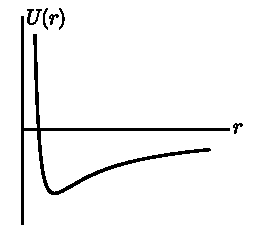
\includegraphics[width=4cm]{fig11.pdf}\\[0.3em]{\small 图 11}\end{minipage}\par\nopagebreak

引入下列新变量：
\begin{equation*}
  \rho=\frac{2\sqrt{-2mE}}{\hbar}\,r,
\end{equation*}
并令
\begin{equation}
  \frac{2mA}{\hbar^2}+l(l+1)=s(s+1),
\end{equation}
\begin{equation}
  \frac{B}{\hbar}\sqrt{\frac{m}{-2E}}=n.
\end{equation}
则(1)式呈下列形式：
\begin{equation*}
  R''+\frac{2}{\rho}R'
  +\left(-\frac{1}{4}+\frac{n}{\rho}-\frac{s(s+1)}{\rho^2}\right)R=0,
\end{equation*}
这和(36.4)具有同一形式.因此可以立刻断定，满足所需条件的解为
\begin{equation*}
  R=\rho^s\mathrm{e}^{-\rho/2}\,\mathrm{F}(-n+s+1,2s+2,\rho),
\end{equation*}
其中的 $n-s-1=p$ 必须是一个正整数（或零），并且 $s$ 必须取(2)式的正根.按定义(3)，我们得知其能级为
\begin{equation*}
  -E_p=\frac{2B^2m}{\hbar^2}
  \left[2p+1+\sqrt{(2l+1)^2+\frac{8mA}{\hbar^2}}\right]^{-2}.
\end{equation*}

\noindent{\heiti 习题4}\quad 同上题，但 $U=\frac{A}{r^2}+Br^2$（图12）.

解：此题只有离散谱.薛定谔方程如下：
\begin{equation*}
  \frac{\mathrm{d}^2R}{\mathrm{d}r^2}+\frac{2}{r}\frac{\mathrm{d}R}{\mathrm{d}r}
  +\frac{2m}{\hbar^2}\left[E-\frac{\hbar^2l(l+1)}{2mr^2}
  -\frac{A}{r^2}-Br^2\right]R=0.
\end{equation*}
引入变量
\begin{equation*}
  \xi=\frac{\sqrt{2mB}}{\hbar}\,r^2,
\end{equation*}
并令
\begin{equation*}
  l(l+1)+\frac{2mA}{\hbar^2}=2s(2s+1),
\end{equation*}
\begin{equation*}
  \sqrt{\frac{2m}{B}}\,\frac{E}{\hbar}=4(n+s)+3,
\end{equation*}

\par\nopagebreak\noindent\begin{minipage}{\linewidth}\centering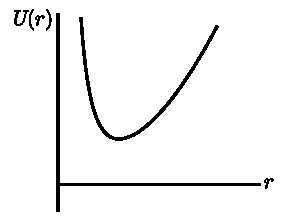
\includegraphics[width=4.5cm]{fig12.pdf}\\[0.3em]{\small 图 12}\end{minipage}\par\nopagebreak

得方程
\begin{equation*}
  \xi R''+\frac{3}{2}R'
  +\left[n+s+\frac{3}{4}-\frac{\xi}{4}-\frac{s\left(s+\frac{1}{2}\right)}{\xi}\right]R=0.
\end{equation*}
当 $\xi\to\infty$ 时，所求解的渐近行为如 $\mathrm{e}^{-\xi/2}$，而当 $\xi$ 很小时，这个解应和 $\xi^s$ 成正比，其中的 $s$ 必须取正值
\begin{equation*}
  s=\frac{1}{4}\left[-1+\sqrt{(2l+1)^2+\frac{8mA}{\hbar^2}}\right].
\end{equation*}
因此，可令所求解呈下列形式：
\begin{equation*}
  R=\mathrm{e}^{-\xi/2}\xi^s w,
\end{equation*}
则得 $w$ 的方程为
\begin{equation*}
  \xi w''+\left(2s+\frac{3}{2}-\xi\right)w'+nw=0,
\end{equation*}
从而得
\begin{equation*}
  w=\mathrm{F}\left(-n,2s+\frac{3}{2},\xi\right),
\end{equation*}
其中的 $n$ 必须取非负整数.因而发现所得的能级是等间隔的无穷集合：
\begin{equation*}
  E_n=\hbar\sqrt{\frac{B}{2m}}
  \left[4n+2+\sqrt{(2l+1)^2+\frac{8mA}{\hbar^2}}\right],
  \quad n=0,1,2,\cdots.
\end{equation*}

\end{xiti}
\renewcommand{\theequation}{\arabic{section}.\arabic{equation}}%

\section{库仑场中的运动（抛物坐标）}

对任意有心力场中的运动而言，薛定谔方程在球坐标中总能够分离变量.在库仑场的情形下，这种分离变量法也能在抛物坐标系中实现.库仑场问题在抛物坐标系中的解，对于某些问题的研究特别有用，这些问题中的某一空间方向具有特殊性；例如，处于外电场中的一个原子（见§77）.

抛物坐标系 $\xi$，$\eta$，$\varphi$ 是由下式定义的：
\begin{equation}
\begin{aligned}
  &x=\sqrt{\xi\eta}\cos\varphi,\qquad
  y=\sqrt{\xi\eta}\sin\varphi,\qquad
  z=\frac{1}{2}(\xi-\eta),\\
  &r=\sqrt{x^2+y^2+z^2}=\frac{1}{2}(\xi+\eta).
\end{aligned}
\end{equation}
或反之：
\begin{equation}
  \xi=r+z,\qquad\eta=r-z,\qquad
  \varphi=\arctan\left(\frac{y}{x}\right);
\end{equation}
$\xi$ 和 $\eta$ 的取值可以从0到 $\infty$，$\varphi$ 是从0到 $2\pi$.曲面 $\xi=$ 常数和 $\eta=$ 常数，都是绕 $z$ 轴的旋转抛物面，并以原点为焦点.这是一套正交坐标系.长度元由下式给出：
\begin{equation}
  (\mathrm{d}l)^2=\frac{\xi+\eta}{4\xi}(\mathrm{d}\xi)^2
  +\frac{\xi+\eta}{4\eta}(\mathrm{d}\eta)^2+\xi\eta(\mathrm{d}\varphi)^2,
\end{equation}
体积元为
\begin{equation}
  \mathrm{d}V=\frac{1}{4}(\xi+\eta)\,\mathrm{d}\xi\,\mathrm{d}\eta\,\mathrm{d}\varphi.
\end{equation}
由(37.3)式，拉普拉斯算符可表为
\begin{equation}
  \Delta=\frac{4}{\xi+\eta}\left[\frac{\partial}{\partial\xi}
  \left(\xi\frac{\partial}{\partial\xi}\right)
  +\frac{\partial}{\partial\eta}
  \left(\eta\frac{\partial}{\partial\eta}\right)\right]
  +\frac{1}{\xi\eta}\frac{\partial^2}{\partial\varphi^2}.
\end{equation}
库仑引力场
\begin{equation*}
  U=-\frac{1}{r}=-\frac{2}{\xi+\eta}
\end{equation*}
中的单粒子薛定谔方程呈以下形式：
\begin{equation}
  \frac{4}{\xi+\eta}\left[\frac{\partial}{\partial\xi}
  \left(\xi\frac{\partial\psi}{\partial\xi}\right)
  +\frac{\partial}{\partial\eta}
  \left(\eta\frac{\partial\psi}{\partial\eta}\right)\right]
  +\frac{1}{\xi\eta}\frac{\partial^2\psi}{\partial\varphi^2}
  +2\left(E+\frac{2}{\xi+\eta}\right)\psi=0.
\end{equation}
令本征函数 $\psi$ 呈下列形式：
\begin{equation}
  \psi=f_1(\xi)f_2(\eta)\,\mathrm{e}^{im\varphi},
\end{equation}
其中的 $m$ 是磁量子数.上式代入(37.6)并乘以 $\frac{1}{4}(\xi+\eta)$，分离 $\xi$ 和 $\eta$ 变量，得 $f_1$ 和 $f_2$ 的两个方程式：
\begin{equation}
\left.\begin{aligned}
  \frac{\mathrm{d}}{\mathrm{d}\xi}\left(\xi\frac{\mathrm{d}f_1}{\mathrm{d}\xi}\right)
  +\left[\frac{1}{2}E\xi-\frac{m^2}{4\xi}+\beta_1\right]f_1=0,\\
  \frac{\mathrm{d}}{\mathrm{d}\eta}\left(\eta\frac{\mathrm{d}f_2}{\mathrm{d}\eta}\right)
  +\left[\frac{1}{2}E\eta-\frac{m^2}{4\eta}+\beta_2\right]f_2=0,
\end{aligned}\right\}
\end{equation}
其中的分离参量 $\beta_1$ 和 $\beta_2$ 的关系为
\begin{equation}
  \beta_1+\beta_2=1.
\end{equation}
我们来考虑离散能谱（$E<0$）.引入下列各量代替 $E,\xi,\eta$：
\begin{equation}
  n=\frac{1}{\sqrt{-2E}},\qquad
  \rho_1=\xi\sqrt{-2E}=\frac{\xi}{n},\qquad
  \rho_2=\frac{\eta}{n},
\end{equation}
得 $f_1$ 的方程为
\begin{equation}
  \frac{\mathrm{d}^2f_1}{\mathrm{d}\rho_1^2}
  +\frac{1}{\rho_1}\frac{\mathrm{d}f_1}{\mathrm{d}\rho_1}
  +\left[-\frac{1}{4}+\frac{1}{\rho_1}\left(\frac{|m|+1}{2}+n_1\right)
  -\frac{m^2}{4\rho_1^2}\right]f_1=0,
\end{equation}
对 $f_2$ 可得同样的方程，其中
\begin{equation}
  n_1=-\frac{|m|+1}{2}+n\beta_1,\qquad
  n_2=-\frac{|m|+1}{2}+n\beta_2.
\end{equation}
与求解(36.4)式相似，我们发现，当 $\rho_1$ 很大时 $f_1$ 如同 $\mathrm{e}^{-\frac{1}{2}\rho_1}$，而当 $\rho_1$ 很小时，如同 $\rho_1^{\frac{1}{2}|m|}$.因此可设(37.11)式之解呈下列形式：
\begin{equation*}
  f_1(\rho_1)=\mathrm{e}^{-\frac{1}{2}\rho_1}\rho_1^{\frac{1}{2}|m|}\,w_1(\rho_1)
\end{equation*}
（对 $f_2$ 而言也有类似的式子）.结果得 $w_1$ 的方程：
\begin{equation*}
  \rho_1w_1''+(|m|+1-\rho_1)w_1'+n_1w_1=0.
\end{equation*}
这又是合流超几何函数的方程.满足有限性条件之解为
\begin{equation*}
  w_1=\mathrm{F}(-n_1,|m|+1,\rho_1),
\end{equation*}
其中的 $n_1$ 必须是一个非负整数.

可见在抛物坐标中，离散谱的每一个定态是由这样三个整数确定的：即抛物量子数 $n_1$ 和 $n_2$，以及磁量子数 $m$.对主量子数 $n$ 而言，由(37.9)和(37.12)式得 $n_1$，$n_2$：
\begin{equation}
  n=n_1+n_2+|m|+1.
\end{equation}
至于能级，当然和以前所得的(36.9)式相同.

对给定的 $n$ 而言，$|m|$ 可取0到 $n-1$，共 $n$ 个不同的数值.固定 $n$ 和 $|m|$ 以后，$n_1$ 尚可取 $n-|m|$ 个不同的数值，从0到 $n-|m|-1$.再考虑到对给定的 $|m|$ 我们可以选取 $m=\pm|m|$ 两种不同的函数.因此，对一个给定的 $n$ 值而言，一共有
\begin{equation*}
  2\sum_{m=1}^{n-1}(n-m)+(n-0)=n^2
\end{equation*}
个不同的态，这和§36中所得的结论一致.

离散谱的波函数 $\psi_{n_1n_2m}$ 应按下列条件归一化：
\begin{equation}
  \int|\psi_{n_1n_2m}|^2\,\mathrm{d}V
  =\frac{1}{4}\int_0^{\infty}\int_0^{\infty}\int_0^{2\pi}
  |\psi_{n_1n_2m}|^2(\xi+\eta)\,\mathrm{d}\xi\,\mathrm{d}\eta\,\mathrm{d}\varphi=1.
\end{equation}
归一化后的波函数具有下列形式：
\begin{equation}
  \psi_{n_1n_2m}=\frac{\sqrt{2}}{n^2}\,
  f_{n_1m}\left(\frac{\xi}{n}\right)f_{n_2m}\left(\frac{\eta}{n}\right)
  \frac{\mathrm{e}^{im\varphi}}{\sqrt{2\pi}},
\end{equation}
其中
\begin{equation}
  f_{pm}(\rho)=\frac{1}{|m|!}\sqrt{\frac{(p+|m|)!}{p!}}\,
  \mathrm{F}(-p,|m|+1,\rho)\,\mathrm{e}^{-\frac{1}{2}\rho}\rho^{\frac{1}{2}|m|}.
\end{equation}
与球坐标中的不同，抛物坐标中的波函数对 $z=0$ 的平面是不对称的.$n_1>n_2$ 时，发现粒子的概率在 $z>0$ 的方向大于 $z<0$ 的方向，$n_1<n_2$ 时则反之.

连续谱（$E>0$）情形下，(37.8)式中的 $\beta_1$ 和 $\beta_2$ 参量都取实的连续值［当然仍有(37.9)式的关系］.我们不准备把这种情形下的波函数写出来，因为通常不大用到.如果把(37.8)式看作“本征值”$\beta_1$ 和 $\beta_2$ 所应满足的方程式，则 $\beta_1$ 和 $\beta_2$ 还可以取复数值（$E>0$ 时）.与此相应的波函数将在§135中写出，我们在该节中利用它们去求解库仑场中的散射问题.

定态 $|n_1n_2m\rangle$ 的存在导致一个附加守恒律(36.29).在这些态中，能量以及量 $l_z=m$ 和 $A_z$ 均有定值.计算算符 $\hat{A}_z$ 的对角矩阵元，给出
\begin{equation}
  A_z=\frac{n_1-n_2}{n}.
\end{equation}
其中 $u_z=n_1-n_2$，“角动量”$j_1$ 和 $j_2$ 的分量值为
\begin{equation}
\left.\begin{aligned}
  j_{1z}&=\frac{1}{2}(m+n_1-n_2)\equiv\mu_1,\\
  j_{2z}&=\frac{1}{2}(m-n_1+n_2)\equiv\mu_2.
\end{aligned}\right\}
\end{equation}
根据 $|n_1n_2m\rangle$ 态（即 $|n\mu_1\mu_2\rangle$ 态）的这些性质容易建立起它们与 $|nlm\rangle$ 态之间波函数的关系.由于 $\boldsymbol{l}=\boldsymbol{j}_1+\boldsymbol{j}_2$，这两个表象间的相互变换，基本上就是§106中讨论的两个角动量相加时的波函数组合问题.所以用“角动量”$j_1$ 和 $j_2$ 来表述时，$|nlm\rangle$ 和 $|n_1n_2m\rangle$ 态可写为 $|j_1j_2lm\rangle$ 和 $|j_1j_2\mu_1\mu_2\rangle$ 态，根据(36.35)和(37.13)，我们有
\begin{equation}
  j_1=j_2=\frac{1}{2}(n-1)=\frac{1}{2}(n_1+n_2+|m|).
\end{equation}
根据一般公式(106.9)—(106.11)，得到（D. Park,1960）
\begin{equation}
\left.\begin{aligned}
  \psi_{nlm}&=\sum_{\mu_1+\mu_2=m}
  \langle lm\mid\mu_1\mu_2\rangle\,\psi_{n\mu_1\mu_2},\\
  \psi_{n\mu_1\mu_2}&=\sum_{l=0}^{n-1}
  \langle l,\mu_1+\mu_2\mid\mu_1\mu_2\rangle\,\psi_{nlm}.
\end{aligned}\right\}
\end{equation}